\icode{N23J-ME-SI-L3-261016-001}
\nceeID[3]{2023北京}{11}
如图所示，一物体在力 \( F \) 作用下沿水平桌面做匀加速直线运动。已知物体质量为 \( m \)，加速度大小为 \( a \)，物体和桌面之间的动摩擦因数为 \( \mu \)，重力加速度为 \( g \)。在物体移动距离为 \( x \) 的过程中\paren[]
	
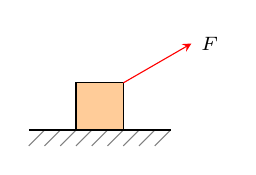
\begin{tikzpicture}[>=stealth,font=\scriptsize]
	\draw[fill=orange!40] (0,0) rectangle(.6,.6);
	\draw[->,red] (.6,.6)--++(30:1)node[right,black]{\(F\)};
	\foreach \x in {-.6,-.4,...,1.2}
		\draw[gray] (\x,-.2)--++(.2,.2);
	\draw[thick] (-.6,0)--(1.2,0);
\end{tikzpicture}
\begin{choices}
	\item 摩擦力做功大小与 \( F \) 方向无关
	\item 合力做功大小与 \( F \) 方向有关
	\item \( F \) 为水平方向时，\( F \) 做功为 \( \mu mgx \)
	\item \( F \) 做功的最小值为 \( max  \)
\end{choices}
\begin{answer}
	D\qquad 提示：\(W_F - W_f = F _{\text{合}}\cdot x =ma\cdot x\)
\end{answer}